% +------------------------------------------------------------------------+
% | Reference manual page: Triangulation_2.tex
% +------------------------------------------------------------------------+
% | 29.03.2000   YVINEC
% | Package: Triangulation
% | 
\RCSdef{\RCSTriangulationRev}{$Revision$}
\RCSdefDate{\RCSTriangulationDate}{$Date$}
% |
%%RefPage: end of header, begin of main body
% +------------------------------------------------------------------------+


\ccModifierCrossRefOff
\begin{ccRefClass}{Triangulation_2<Traits,Tds>}  %% add template arg's if necessary

%% \ccHtmlCrossLink{}     %% add further rules for cross referencing links
%% \ccHtmlIndexC[class]{} %% add further index entries

\ccDefinition
  
The class \ccRefName\ is the basic class 
designed to handle triangulations
of set of points ${  A}$ in the plane.

Such a triangulation has vertices at the points of ${  A}$
and its domain covers the convex hull of ${  A}$.
It can be viewed as a planar partition of the plane
whoses bounded faces are triangular and cover
the convex hull of ${  A}$. The single unbounded face of this partition
is the complementary of the convex hull of ${  A}$.
 
In many applications, it is convenient to
deal only with triangular faces. Therefore, we add to the
triangulation
a fictitious vertex, called the \ccc{infinite vertex}
and we make each  convex hull edge incident 
to an \ccc{infinite} 
face having as third vertex  the \ccc{infinite vertex}.
 In that way, each edge is incident to exactly two faces
and special cases at the
boundary of the convex hull are simpler to deal with.

\begin{figure}[h]
\begin{ccTexOnly}
\begin{center} 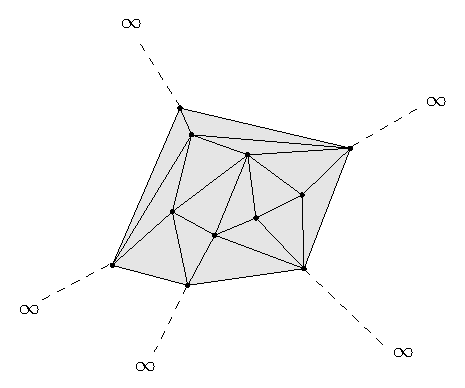
\includegraphics[scale=0.5]{Triangulation_2_ref/infinite_vertex} \end{center}
\end{ccTexOnly}
\caption{The infinite vertex.
\label{Triangulation_ref_Fig_infinite_vertex}}
\begin{ccHtmlOnly}
<CENTER>
<img border=0 src=infinite_vertex.gif align=center alt="Vertices at
infinity">
</CENTER>
\end{ccHtmlOnly}
\end{figure}

The class \ccRefName\
implements this point of view
and therefore considers  the triangulation of the set of points 
as a set of  triangular,  finite and
infinite faces. 
Although it is convenient to draw a triangulation as in
figure~\ref{Triangulation_ref_Fig_infinite_vertex}, note that
the \ccc{infinite vertex} has no significant
coordinates and that no geometric predicate can be applied on it
or on an infinite face.

A triangulation is a collection of vertices and faces that
are linked together through incidence and adjacency relations.
Each face give access to its three incident vertices and to
its 
three adjacent faces. Each vertex give access to one of its  incident
faces. 

The three vertices of a face are indexed with 0, 1 and 2
in counterclockwise order. The neighbor of a face are also 
indexed with 0,1,2 in such a way that the neighbor indexed by $i$
is opposite to the vertex with the same index.

The triangulation class
offer  two functions \ccStyle{int cw(int i)} and 
\ccStyle{int ccw(int i)} 
which given the index of a vertex in a face
compute the index of the next vertex  of the same face
in clockwise
or counterclockwise order.
 Thus, for example the neighbor 
\ccc{neighbor(cw(i))} is
 the
neighbor of \ccc{f}  which is next to \ccc{neighbor(i)} turning clockwise
around \ccc{f}. The face \ccc{neighbor(cw(i))}
is also the first face encountered after \ccc{f} when
turning clockwise around vertex \ccc{i}
of~\ccc{f} (see Figure~\ref{Triangulation_ref_Fig_neighbors}).



 \begin{figure}
\begin{ccTexOnly}
    \begin{center}
     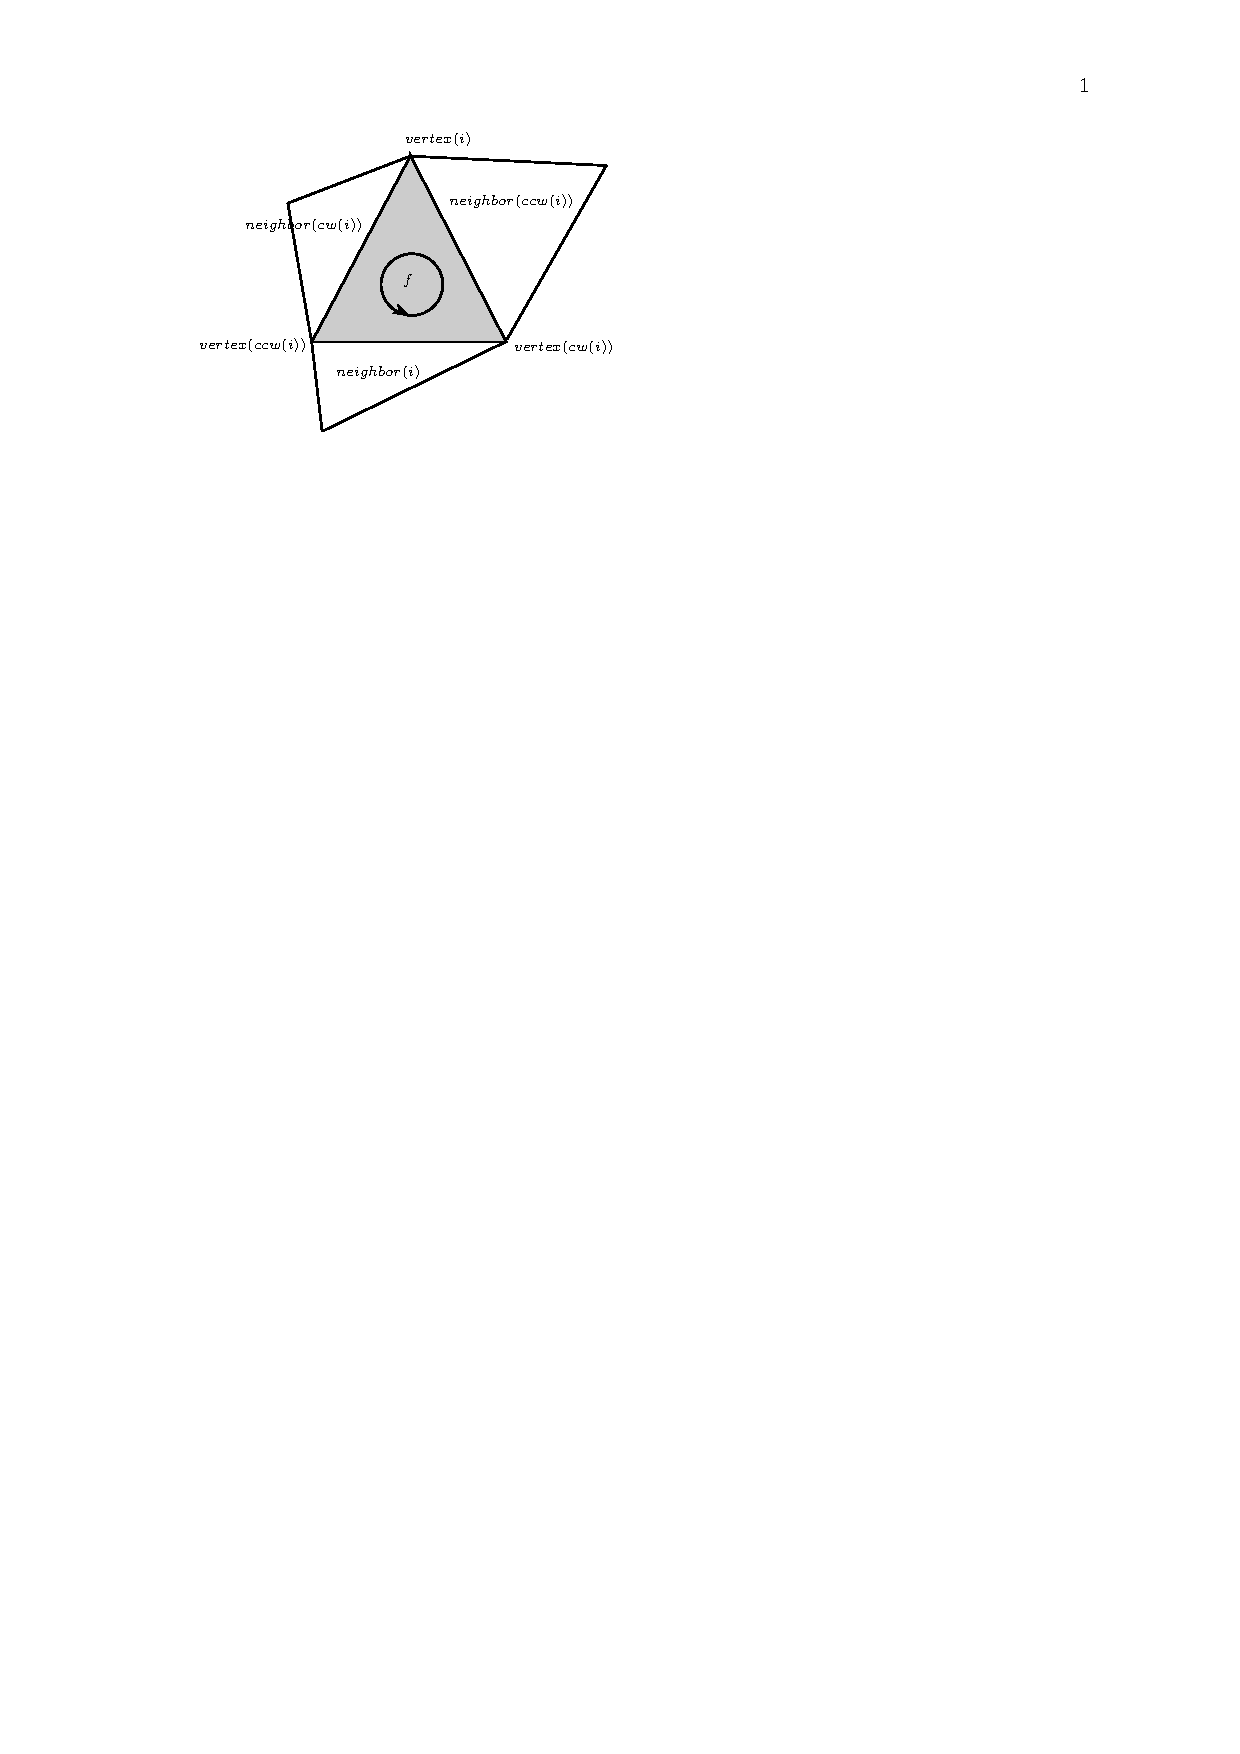
\includegraphics{Triangulation_2/neighbors}
    \end{center}
\end{ccTexOnly} 
    \caption{Vertices and neighbors.
    \label{Triangulation_ref_Fig_neighbors}}
  \begin{ccHtmlOnly}
<CENTER>
<img border=0 src=neighbors.gif align=center alt="Neighbors">
</CENTER>
\end{ccHtmlOnly} 
\end{figure}



\ccInclude{CGAL/Triangulation_2.h}

\ccParameters
The class \ccRefName\ has  two template parameters. The first one
\ccc{Traits} is the geometric traits, it is to be instantiated by
 a model of the concept \ccc{TriangulationTraits_2}.

The second parameter is the triangulation data structure,
it has to be instantiated by a model of the concept
\ccc{TriangulationDataStructure_2}.
By befault, the triangulation data structure  is instanciated by
\ccc{CGAL::Triangulation_data_structure_2 <
                       CGAL::Triangulation_vertex_base_2<Gt>,
		       CGAL::Triangulation_face_base_2<Gt> > >}.


\ccInheritsFrom{\ccc{Triangulation_cw_ccw_2}}
This class provides the functions \ccc{cw(i)} et \ccc{ccw(i)}.

\ccTypes
\ccThree{typedef Traits::Triangle_2xxx}{Triangulation_data_structure;}{}
\ccTypedef{typedef Traits Geom_traits;}{the traits class.}
\ccGlue
\ccTypedef{typedef Tds Triangulation_data_structure;}{the triangulation data structure type.}

\ccTypedef{typedef Traits::Point_2t Point;}{the point type}
\ccGlue
\ccTypedef{typedef Traits::Segment_2 Segment;}{the segment type}
\ccGlue
\ccTypedef{typedef Traits::Triangle_2 Triangle;}{the triangle type}

\ccTypedef{typedef Tds::Vertex Vertex;}{the vertex type.}
\ccGlue
\ccTypedef{typedef Tds::Face Face;}{the face type.}
\ccGlue
\ccTypedef{typedef Tds::Edge  Edge;} {the edge type.}

\ccTypedef{typedef Tds::size_type size_type;}
{Size type (an unsigned integral type)}
\ccGlue
\ccTypedef{typedef Tds::difference_type difference_type;}
{Difference type (a signed integral type)}

\ccThree{typedef Traits::Triangle_2xxx}{}{the triangulation data structure type}
\ccThreeToTwo
The vertices and faces of the triangulations are accessed through 
\ccc{handles}, 
\ccc{iterators} and \ccc{circulators}. 
The  handles are models of the concept \ccc{Handle} which basically
offers the two dereference operators \ccc{*} and \ccc{->}.
The iterators and circulators
are all bidirectional and non mutable.
The circulators and iterators are convertible  to handles with the
same value type, so that whenever a handle appear in the parameter 
list of a function, an appropriate iterator or circulator can be passed
as well.

The edges of the triangulation can also be visited through iterators
and circulators,
the edge circulators and iterators
are also bidirectional and non mutable.

In the following, we called {\it infinite} any face or edge 
incident  to the infinite vertex and the infinite vertex itself.
 Any other feature (face, edge or vertex) of the triangulation is said 
to be {\it finite}.
Some iterators (the \ccc{All} iterators ) allows to visit finite or 
infinite feature while others (the \ccc{Finite} iterators) visit only
finite features. Circulators visit infinite features as well as finite 
ones.

\ccTypedef{typedef Tds::Vertex_handle Vertex_handle;}
{handle to a vertex}
\ccGlue
\ccTypedef{typedef Tds::Face_handle Face_handle;}
{handle to a face}


\ccTypedef{typedef Tds::Face_iterator All_faces_iterator;}
{iterator over all faces.}
\ccGlue
\ccTypedef{typedef Tds::Edge_iterator All_edges_iterator;}
{iterator over all edges}
\ccGlue
\ccTypedef{typedef Tds::Vertex_iterator All_vertices_iterator;}
{iterator over all vertices}

\ccNestedType{Finite_faces_iterator}{iterator over finite faces.}
\ccGlue
\ccNestedType{Finite_edges_iterator
}{iterator over finite edges.}
\ccGlue
\ccNestedType{Finite_vertices_iterator}{iterator over finite
vertices.}
\ccGlue
\ccNestedType{Point_iterator}{iterator over the points corresponding the
finite vertices of the triangulation.} 


\ccNestedType{Line_face_circulator}{circulator over all faces intersected by a line.}


\ccNestedType{Face_circulator} 
{circulator over all faces incident to a given vertex.}
\ccGlue
\ccNestedType{Edge_circulator}
{circulator over all  edges incident to a given vertex.}
\ccGlue
\ccNestedType{Vertex_circulator}
{circulator over all vertices incident to a given vertex.}

The triangulation class also defines the following enum type to specify
which case occurs when locating a point in the triangulation.

\ccEnum{enum Locate_type {VERTEX=0, EDGE, FACE, OUTSIDE_CONVEX_HULL,
OUTSIDE_AFFINE_HULL};}{The locate type is \ccc{OUTSIDE_CONVEX_HULL} when the point
is  outside the convex hull but in the affine hull of the current triangulation. \\
The locate type is \ccc{OUTSIDE_AFFINE_HULL} 
when the point is outside the affine hull
of the current triangulation.}


\ccCreation
\ccCreationVariable{t}  %% choose variable name



\ccThree{Triangulation_2<>}{t = Triangulation_2 tr}{}
\ccThreeToTwo
\ccConstructor{Triangulation_2();}{default constructor.}
\ccGlue
\ccConstructor{Triangulation_2(
                   const Traits& gt = Traits() );}
{Introduces an empty triangulation \ccVar.}


\ccConstructor{Triangulation_2(
                   const Triangulation_2& tr);}
{Copy constructor. All the vertices and faces are duplicated.
 After the copy, \ccVar\ and \ccc{tr}
refer to different triangulations~: 
 if \ccc{tr} is modified, \ccVar\ is not. }

\ccMethod{Triangulation_2 operator=(const Triangulation_2& tr);}
{Assignement. All the vertices and faces are duplicated.
 After the assignement, \ccVar\ and \ccc{tr}
refer to different triangulations~: 
 if \ccc{tr} is modified, \ccVar\ is not.}

\ccThree{Vertex_handle}{t.number_of_vertices()x}{}
\ccMethod{void swap(Triangulation_2& tr);}
{The triangulations \ccc{tr} and \ccVar\ are swapped.
\ccc{t.swap(tr)} should be preferred to \ccc{t} = \ccc{tr} or to
\ccc{t(tr)} if \ccc{tr} is deleted after that.}

\ccMethod{void clear();}{Deletes all faces and finite vertices
resulting
 in an
empty triangulation.}

\ccFunction{void ~Triangulation_2();}
{Destructor. All vertices and faces are deleted.}


\ccAccessFunctions
\ccMethod{const Geom_traits& geom_traits() const;}
{Returns a const reference to the triangulation traits object.}
\ccGlue
\ccMethod{const TriangulationDataStructure_2 & tds() const;}
{Returns a const reference to the triangulation data structure.}

\begin{ccAdvanced}
\ccHeading{Non const access}
The responsibility of keeping a valid triangulation belongs to the user
when using advanced operations allowing a direct manipulation of the \ccc{tds}.

\ccMethod{TriangulationDataStructure_2 & tds();}
{Returns a reference to the triangulation data structure.}

This method is mainly a help for users implementing their own triangulation
algorithms.
 
\end{ccAdvanced}


\ccGlue
\ccMethod{int dimension() const;}
{Returns the dimension of the convex hull.}
\ccGlue
\ccMethod{size_type number_of_vertices() const;}
{Returns the number of finite vertices.}
\ccGlue
\ccMethod{size_type number_of_faces() const;}
{Returns the number of finite faces.}

\ccMethod{Face_handle infinite_face() const;}
{a  face incident to the \ccc{infinite_vertex}.}
\ccGlue
\ccMethod{Vertex_handle
          infinite_vertex();}
{the \ccc{infinite_vertex}.}
\ccGlue
\ccMethod{Vertex_handle finite_vertex() const;}
{a vertex distinct from  the \ccc{infinite_vertex}.}


\ccPredicates
The class \ccRefName\ provides methods to test
the finite or infinite character of any feature,
and also methods to test the presence in the triangulation
of a particular feature (edge or face).

\ccThree{bool }{t.is_infinite( Face_handle f, int i)x}{}
\ccMethod{bool
          is_infinite(Vertex_handle v) const;}
{\ccc{true} iff \ccc{v} is the \ccc{infinite_vertex}.}
\ccGlue
\ccMethod{bool
          is_infinite(Face_handle f) const;}
{\ccc{true} iff face \ccc{f} is infinite.}
\ccGlue
\ccMethod{bool is_infinite(Face_handle f, int i) const;}
{\ccc{true} iff edge \ccc{(f,i)} is infinite.}
\ccGlue
\ccMethod{bool
          is_infinite(Edge e) const;}
{\ccc{true} iff edge \ccc{e} is infinite.}
\ccGlue
\ccMethod{bool
          is_infinite(Edge_circulator ec) const;}
{\ccc{true} iff edge \ccc{*ec} is infinite.}
\ccGlue
\ccMethod{bool
          is_infinite(Edge_iterator ei) const;}
{\ccc{true} iff edge \ccc{*ei} is infinite.}


\ccMethod{bool is_edge(Vertex_handle va, Vertex_handle vb);}
{\ccc{true} if there is an edge having \ccc{va} and \ccc{vb} as
vertices.}
\ccGlue
\ccMethod{bool is_edge(Vertex_handle va, Vertex_handle vb, Face_handle& fr,
	       int & i);}
{ as above. In addition, if \ccc{true} is returned,  the edge with
vertices \ccc{va} and \ccc{vb} is the edge \ccc{e=(fr,i)} where
\ccc{fr} is a handle to the face incident to \ccc{e} and 
on the right side of  \ccc{e} oriented from \ccc{va} to \ccc{vb}.}
\ccGlue
\ccMethod{bool includes_edge(Vertex_handle va, Vertex_handle & vb,
		     Face_handle& fr, int & i);}
{\ccc{true} if the line segment from \ccc{va} to \ccc{vb} includes
an edge \ccc{e} incident to \ccc{va}. If \ccc{true}, \ccc{vb} becomes
the other vertex of \ccc{e}, \ccc{e} is the edge \ccc{(fr,i)} where
\ccc{fr} is a handle to the face incident to \ccc{e} and 
on the right side \ccc{e} oriented from \ccc{va} to \ccc{vb}.}
\ccGlue
\ccMethod{bool is_face(Vertex_handle v1, Vertex_handle v2, Vertex_handle v3);}
{\ccc{true} if there is a face having \ccc{v1}, \ccc{v2} and \ccc{v3} 
as vertices.}
\ccGlue
\ccMethod{bool is_face(Vertex_handle v1, Vertex_handle v2, Vertex_handle v3,
      Face_handle &fr);}
{as above. In addition, if \ccc{true} is returned, fr is a handle
to the face with  \ccc{v1}, \ccc{v2} and \ccc{v3} 
as vertices.} 

\ccHeading{Queries}

The class \ccRefName\  provides methods to locate
a given point with respect to a triangulation. It also provides
methods to locate a point with respect to
a given  finite face of the triangulation.

\ccThree{Vertex_handle}{t.locate(Point query,}{}
\ccMethod{Face_handle
          locate(const Point& query,
                 Face_handle f = Face_handle()) const;}
{If the point \ccc{query} lies inside the convex hull of the points, a face 
that contains the query in its interior or on its
 boundary is returned.\\
If the point \ccc{query} lies outside the convex hull of the
triangulation but in the affine hull,
the returned face is an infinite face which is a proof of the point's
location : \\
- for a two dimensional triangulation, it is a face $(\infty, p, q)$ 
such that
\ccc{query} lies to the left  of the oriented line $pq$ 
(the rest of the triangulation lying to the right of this line).\\
- for a degenerate one dimensional triangulation it is the (degenarate
one dimensional) face $(\infty, p, NULL)$ such that \ccc{query}
and the triangulation lie on either side of \ccc{p}. \\
If the point \ccc{query} lies outside the affine hull,
the returned \ccc{Face_handle} is \ccc{NULL}. \\
The optional \ccc{Face_handle} argument, if provided, is used as a hint
of where the locate process has to start its search.}

\ccMethod{Face_handle
          locate(const Point& query,
                 Locate_type& lt,
                 int& li,
                 Face_handle h =Face_handle() ) const;}
{Same as above. Additionally, the parameters \ccc{lt}
 and \ccc{li}
describe where the query point is located. 
The variable \ccc{lt} is set to the locate type of the query.
If \ccc{lt==VERTEX} 
the variable \ccc{li}
is set to the index of the vertex, and if \ccc{lt==EDGE}
\ccc{li}
is set to the index 
of the vertex opposite to the
edge. 
Be careful that \ccc{li}
has no meaning when the query type is \ccc{FACE}, \ccc{OUTSIDE_CONVEX_HULL}, 
or \ccc{OUTSIDE_AFFINE_HULL} or when the
triangulation is $0$-dimensional.}

\ccMethod{Oriented_side
           oriented_side(Face_handle f,
                         const Point& p) const;}
{Returns on which side of the oriented boundary of \ccc{f} lies 
the point \ccc{p}. \ccPrecond \ccc{f} is finite.}

\ccMethod{Oriented_side
 side_of_oriented_circle(Face_handle f, const Point & p);}
{Returns on which side of the circumcircle  of face \ccc{f} lies 
the point \ccc{p}. The circle is assumed to be counterclockwisely
oriented, so its positive
side correspond to its bounded side.
This predicate is available only if the corresponding predicates on
points is provided in the geometric traits class.}

\ccHeading{Modifiers}

The following operations are guaranteed to lead to a valid triangulation 
when they are applied on a valid triangulation.

\ccMethod{void flip(Face_handle f, int i);}{Exchanges the edge incident to
\ccc{f} and \ccc{f->neighbor(i)} with the other
diagonal of the quadrilateral formed by \ccc{f} and  \ccc{f->neighbor(i)}.
\ccPrecond {The faces \ccc{f} and \ccc{f->neighbor(i)} are finite faces
and their union form a convex quadrilateral.}}



\ccMethod{Vertex_handle insert(const Point& p,
                         Face_handle f = Face_handle());}
{Inserts point \ccc{p} in the triangulation and returns the corresponding
 vertex.\\
If point \ccc{p} coincides with an already existing vertex, this 
vertex is returned and the triangulation remains unchanged.\\
If point \ccc{p} is on an edge, the two incident faces are split 
in two.\\
If point \ccc{p} is strictly inside a face of the triangulation,
the face is split in three.\\
If point \ccc{p} is strictly outside the  convex hull, \ccc{p} is linked
to all visible points on the convex hull to form the new
triangulation.\\
At last, if \ccc{p} is outside the affine hull (in case of degenerate
1-dimensional or 0-dimensional triangulations), \ccc{p}
is linked all the  other vertices to form a triangulation whose
dimension is increased by one.
The last argument \ccc{f} is an indication to the underlying locate
algorithm of where to start.
}


\ccMethod{Vertex_handle 
          insert(const Point& p,
                 Locate_type lt,
                 Face_handle loc, int li );}
{Same as above except that the location of the point
 \ccc{p} to be inserted is assumed to be given by
\ccc{(lt,loc,i)} (see the description of the \ccc{locate} method above.)}

\ccMethod{Vertex_handle push_back(const Point& p);}
{Equivalent to \ccc{insert(p)}.}

\ccMethod{template < class InputIterator >
          int
          insert(InputIterator first, InputIterator last);}
{Inserts the points in the range
 $\left[\right.$\ccc{first}, \ccc{last}$\left.\right)$.
 Returns the number of inserted points.
 \ccPrecond The \ccc{value_type} of \ccc{InputIterator}
 is \ccc{Point}.}

\ccMethod{void    remove(Vertex_handle v);}
{Removes the vertex from the triangulation. The created hole is 
 retriangulated.
 \ccPrecond Vertex \ccc{v} must be finite.}


\begin{figure}
\begin{ccTexOnly}
\begin{center}
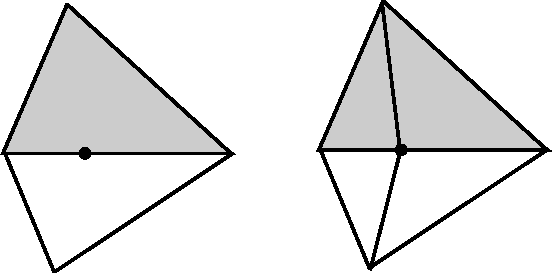
\includegraphics{Triangulation_2/insert1}
\end{center}
\end{ccTexOnly}
\caption{Insertion of a point on an edge.
\label{Triangulation_ref_Fig_inser1t}}

\begin{ccHtmlOnly}
<CENTER>
<img border=0 src=insert1.gif align=center alt="Insertion in an edge">
</CENTER>
\end{ccHtmlOnly}
\end{figure}




\begin{figure}
\begin{ccTexOnly}
\begin{center}
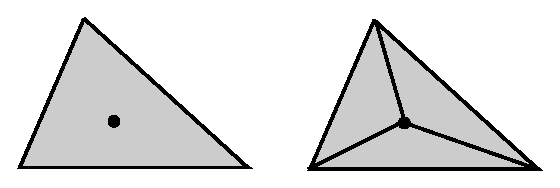
\includegraphics{Triangulation_2/insert2}
\end{center}
\end{ccTexOnly}
\caption{Insertion in a face.
\label{Triangulation_ref_Fig_insert2}}

\begin{ccHtmlOnly}
<CENTER>
<img border=0 src=insert2.gif align=center alt="Insertion in a Face">
</CENTER>
\end{ccHtmlOnly}
\end{figure}


\begin{figure}
\begin{ccTexOnly}
\begin{center}
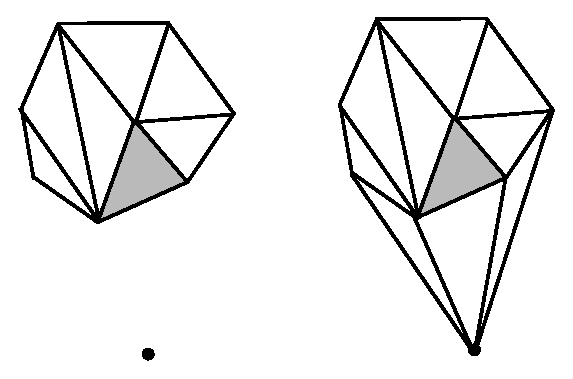
\includegraphics{Triangulation_2/insert3}
\end{center}
\end{ccTexOnly}
\caption{Insertion outside the convex hull.
\label{Triangulation_ref_Fig_insert3}}

\begin{ccHtmlOnly}
<CENTER>
<img border=0 src=insert3.gif align=center alt="Insertion outside the
convex hull">
</CENTER>
\end{ccHtmlOnly}
\end{figure}

\begin{figure}
\begin{ccTexOnly}
\begin{center}
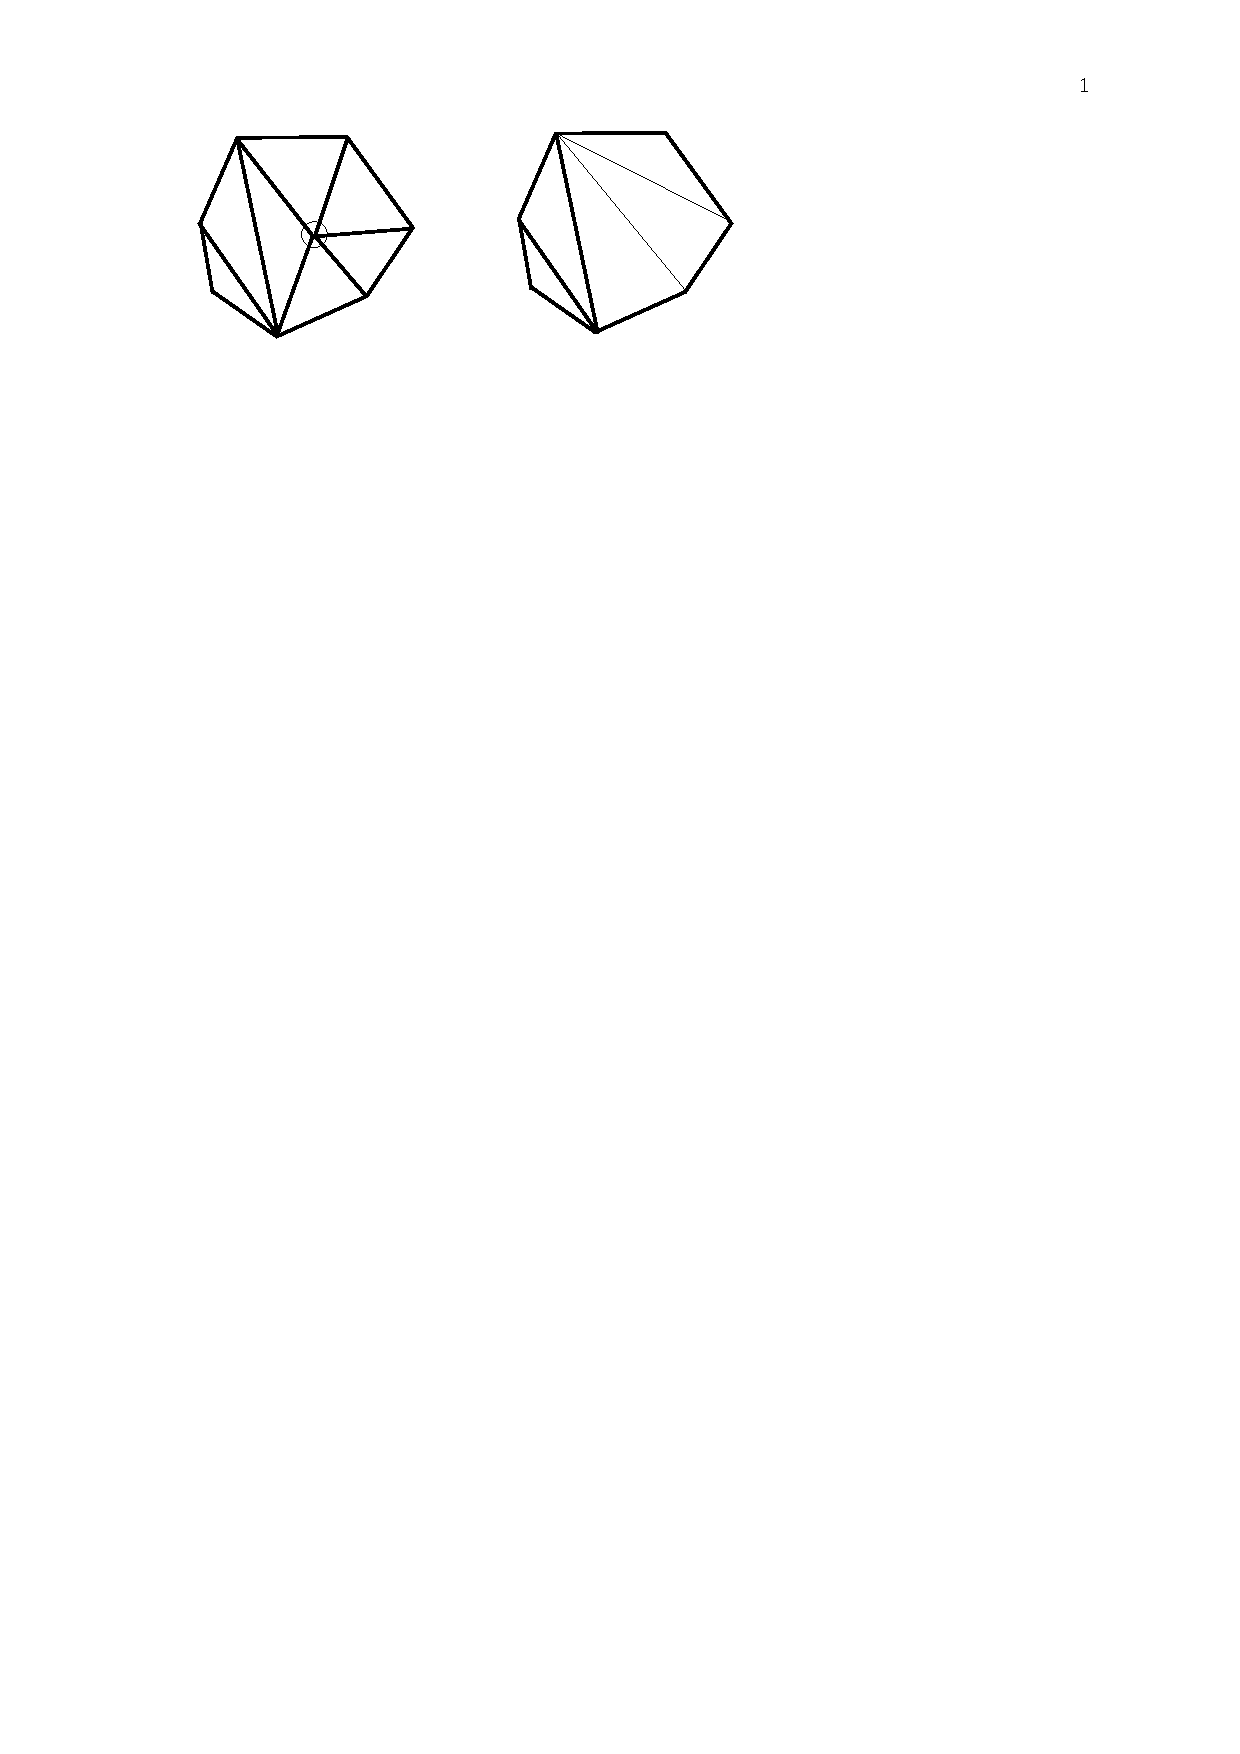
\includegraphics{Triangulation_2/remove}
\end{center}
\end{ccTexOnly}
\caption{Removal
\label{Triangulation_ref_Fig_remove}}

\begin{ccHtmlOnly}
<CENTER>
<img border=0 src=remove.gif align=center alt="Remove">
</CENTER>
\end{ccHtmlOnly}
\end{figure}

\begin{ccAdvanced}
The following member functions offer more specialized versions of the
insertion or removal operations to be used when one knows to be in the
corresponding case.

\ccMethod{Vertex_handle insert_first(const Point& p);} 
{Inserts the first finite  vertex .}
\ccMethod{Vertex_handle insert_second(const Point& p);} 
{Inserts the second finite  vertex .}
\ccMethod{Vertex_handle insert_in_face(const Point& p,Face_handle f);} {Inserts vertex \ccc{v} in face
\ccc{f}. Face \ccc{f} is modified,
two new faces are created.
\ccPrecond{The point in vertex \ccc{v} lies inside face \ccc{f}.}}
\ccMethod{Vertex_handle insert_in_edge(const Point& p, Face_handle f, int i);} 
{Inserts vertex v in edge \ccc{i} of \ccc{f}.
\ccPrecond{The point in vertex \ccc{v} lies on the edge opposite to 
the vertex \ccc{i} of face \ccc{f}.}}
\ccMethod{Vertex_handle insert_outside_convex_hull(const Point& p, Face_handle f);}
{Inserts 
 a point which is outside the convex hull  but in the affine hull.
\ccPrecond{
The handle \ccc{f} points to a face which is a proof  of the location
of\ccc{p}, see the description of the
\ccc{locate} method above.} }
\ccMethod{Vertex_handle insert_outside_affine_hull(const Point& p);}
{Inserts 
 a point which is outside the affine hull.}

\ccMethod{void remove_degree_3(Vertex_handle v);}
{Removes a vertex of degree three. Two of the incident faces are destroyed,
the third one is modified.
\ccPrecond{Vertex
\ccc{v} is a finite vertex with degree three.}}
\ccMethod{void remove_second(Vertex_handle v);}{Removes the before last finite vertex.}
\ccMethod{void remove_first(Vertex_handle v);}{Removes the last finite vertex.}

The following fonctions are mainly intended to be used in conjunction
with the \ccc{find_conflicts()} member fonctions of Delaunay and constrained 
Delaunay triangulations to perform insertions.

\ccMethod{   template<class EdgeIt>
   Vertex_handle star_hole( Point p, 
 			      EdgeIt edge_begin,
 			      EdgeIt edge_end);}
{creates a new vertex \ccc{v} and use it to star the hole 
whose boundary is described  by the sequence of edges \ccc{[edge_begin, 
edge_end[}. Returns a handle to the new vertex.}

\ccMethod{
   template<class EdgeIt, class FaceIt>
   Vertex_handle star_hole( Point p, 
 			      EdgeIt edge_begin,
 			      EdgeIt edge_end,
 			      FaceIt face_begin,
 			      FaceIt face_end);}
{same as above, except that the  algorithm 
first recycles faces in the sequence \ccc{[face_begin, 
face_end[} 
and create new ones only when the sequence is exhausted.}
\end{ccAdvanced}


\ccHeading{Traversal of the Triangulation}


A triangulation can be seen as a container of faces and vertices.
Therefore the triangulation provides several iterators and circulators
that allow to traverse it (completely or partially).



\ccHeading{Face, Edge and Vertex Iterators}

The following iterators allow respectively to visit 
finite faces,  finite edges and  finite vertices
of the triangulation. These iterators are non mutable, bidirectional
and their value types are respectively
\ccc{Face}, \ccc{Edge} and \ccc{Vertex}. 
They are all invalidated by any change in the triangulation.

\ccThree{Finite_vertices_iterator}{t.finite_vertices_begin()x}{}
\ccMethod{Finite_vertices_iterator finite_vertices_begin() const;}{Starts at an arbitrary finite vertex}
\ccGlue
\ccMethod{Finite_vertices_iterator finite_vertices_end() const;}{Past-the-end iterator}

\ccMethod{Finite_edges_iterator finite_edges_begin() const;}{Starts at an arbitrary finite edge}
\ccGlue
\ccMethod{Finite_edges_iterator finite_edges_end() const;}{Past-the-end iterator}

\ccMethod{Finite_faces_iterator finite_faces_begin() const;}{Starts at an arbitrary finite face}
\ccGlue
\ccMethod{Finite_faces_iterator finite_faces_end()
const;}{Past-the-end iterator}
\ccGlue
\ccMethod{Point_iterator points_begin() const;}{}
\ccGlue
\ccMethod{Point_iterator points_end() const;}{Past-the-end iterator}

The following iterators allow respectively to visit all
(finite or infinite) faces, edges and vertices
of the triangulation. These iterators are non mutable, bidirectional
and their value types are respectively
\ccc{Face}, \ccc{Edge} and \ccc{Vertex}. 
They are all invalidated by any change in the triangulation.


\ccMethod{All_vertices_iterator all_vertices_begin() const;}{Starts at an arbitrary  vertex}
\ccGlue
\ccMethod{All_vertices_iterator all_vertices_end() const;}{Past-the-end iterator}

\ccMethod{All_edges_iterator all_edges_begin() const;}{Starts at an arbitrary edge}
\ccGlue
\ccMethod{All_edges_iterator all_edges_end() const;}{Past-the-end iterator}

\ccMethod{All_faces_iterator all_faces_begin() const;}{Starts at an arbitrary face}
\ccGlue
\ccMethod{All_faces_iterator all_faces_end() const;}{Past-the-end iterator}

\ccThree{Line_face_circulator}{T.line_walk(Point p, }{}
\ccHeading{Line Face Circulator}

The triangulation defines a circulator that allows
to visit all faces that are intersected by a line. 
A  face  \ccc{f} is 
considered has being intersected by 
 the oriented line \ccc{l} if either:
\begin{itemize}\ccTexHtml{\itemsep0pt}{}
\item 
\ccc{f} is a finite face whose interior intersects \ccc{l}, or
\item
 \ccc{f} is a finite face with  an edge collinear with \ccc{l} and lies
to the left of \ccc{l}, or
\item
\ccc{f} is an infinite face incident to a  convex hull edge 
whose interior is intersected
by \ccc{l}, or
\item
\ccc{f} is an infinite face incident to a  convex hull vertex
lying on  \ccc{l} and the finite edge of \ccc{f}
lies to the left of \ccc{l}. 
\end{itemize}
The circulator has a singular value if  the line \ccc{l}
intersect no finite face of the triangulation.
This circulator is
non-mutable and bidirectional. Its value type is \ccc{Face}.

\ccMethod{Line_face_circulator
          line_walk(const Point& p,
                    const Point& q,
                    Face_handle f = Face_handle()) const;}
{ This function returns a circulator that allows to visit the 
 faces intersected by the line \ccc{pq}. 
If there is no such face the circulator has a singular value.\\
 The starting point of the circulator is the face \ccc{f}, or, if
 \ccc{f} is omitted,  the first finite face traversed by \ccc{l}. \\
  The circulator wraps around the \ccc{infinite_vertex} :
after the last traversed finite face, it steps through the infinite face adjacent
to this face then through the infinite face adjacent to the first
traversed finite face then through the first finite traversed face
again.
\ccPrecond Points \ccc{p} and \ccc{q} must be different points.
\ccPrecond If \ccc{f != NULL}, the point \ccc{p} must be
inside or on the boundary of \ccc{f}.}

Figure~\ref{Triangulation_ref_Fig_Line_face_circulator} illustrates which finite faces are enumerated. Lines
$l_1$ and $l_2$ have no face to their left. Lines $l_3$ and $l_4$
have faces to their left. Note that the finite faces that are only vertex
incident to lines $l_3$ and  $l_4$ are not enumerated.

\begin{figure}
\begin{ccTexOnly}
\begin{center}  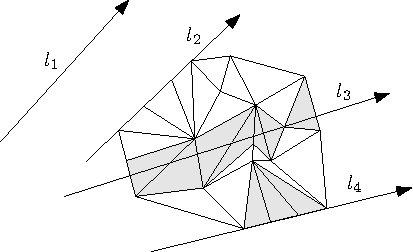
\includegraphics{Triangulation_2/walk} \end{center}
\end{ccTexOnly} 
\caption{The line face circulator.
\label{Triangulation_ref_Fig_Line_face_circulator}}

\begin{ccHtmlOnly}
<CENTER>
<img border=0 src=walk.gif align=center alt="The Infinite Vertex">
</CENTER>
\end{ccHtmlOnly} 
\end{figure}

A line face circulator is invalidated if the face the circulator refers
to is changed.

\ccThree{Vertex_circulator}{t.number_of_vertices()x}{}
\ccThreeToTwo



\ccHeading{Face, Edge and Vertex Circulators}

The triangulation also provides circulators that allows to visit 
respectively all faces or edges incident to a given vertex
or all vertices adjacent to a given vertex.
These circulators are
non-mutable
and bidirectional.
 The \ccc{operator++} moves the circulator
counterclockwise around the vertex while
the \ccc{operator--} moves clockwise.
A face circulator is invalidated by any modification of the face pointed to.
An edge or a vertex circulator are invalidated by any modification
of one of the two faces incident to the edge pointed to.

\ccMethod{Face_circulator incident_faces(Vertex_handle v) const;}
{Starts at an arbitrary face incident
to \ccc{v}.}
\ccGlue
\ccMethod{Face_circulator incident_faces(Vertex_handle v, Face_handle f) const;}
{Starts at face \ccc{f}.
\ccPrecond Face \ccc{f} is incident to vertex \ccc{v}.}
\ccGlue
\ccMethod{Edge_circulator incident_edges(Vertex_handle v) const;}
{Starts at an arbitrary edge incident
to \ccc{v}.}
\ccGlue
\ccMethod{Edge_circulator incident_edges(Vertex_handle v, Face_handle f) const;}
{Starts at the the first edge of \ccc{f} incident to 
\ccc{v}, in counterclockwise order around \ccc{v}.
\ccPrecond Face \ccc{f} is incident to vertex \ccc{v}.}
\ccGlue
\ccMethod{Vertex_circulator incident_vertices(Vertex_handle v) const;}
{Starts at an arbitrary  vertex incident
to \ccc{v}.}
\ccGlue
\ccMethod{Vertex_circulator incident_vertices(Vertex_handle v, Face_handle f) ;}
{Starts at the first vertex of \ccc{f} adjacent  to \ccc{v}
in  counterclockwise order around \ccc{v}.
\ccPrecond Face \ccc{f} is incident to vertex \ccc{v}.}




\ccHeading{Traversal of the Convex Hull}

Applied on the \ccc{infinite_vertex}
the above  functions  allow to visit the vertices on the convex hull and
the infinite edges and faces. Note that a counterclockwise
traversal of the vertices adjacent to the \ccc{infinite_vertex} is
a clockwise traversal of the convex hull.

\ccMethod{Face_circulator incident_faces(t.infinite_vertex()) const;}{}
\ccGlue
\ccMethod{Face_circulator incident_faces(t.infinite_vertex(), Face_handle f) const;}{}
\ccGlue
\ccMethod{Edge_circulator incident_edges(t.infinite_vertex()) const;}{}
\ccGlue
\ccMethod{Edge_circulator incident_edges(t.infinite_vertex(), Face_handle f);}{}
\ccGlue
\ccMethod{Vertex_circulator incident_vertices(t.infinite_vertex() v) ;} {}
\ccGlue
\ccMethod{Vertex_circulator incident_vertices(t.infinite_vertex(), Face_handle f) ;}{}



\ccHeading{Miscellaneous}

\ccThree{Segment}{t.segment(Face_handle f, int i); }{}
\ccMethod{int ccw(int i) const;}
{Returns $i+1$ modulo 3.\ccPrecond $0\leq i \leq 2$.}
\ccGlue
\ccMethod{int cw(int i) const;}
{Returns $i+2$ modulo 3.\ccPrecond $0\leq i \leq 2$.}
\ccGlue
%\ccMethod{int number_of_faces() const;}
%{Returns the number of finite and infinite faces.
%\ccc{TBC_TO} Returns the number of finite faces. This access number functions
%%requires to count the degree 
%of the \ccc{infinite_vertex} and thus is not a constant time access function.}
%\ccGlue
\ccMethod{Triangle
          triangle(Face_handle f) const;}
{Returns the triangle formed by the three vertices of \ccc{f}.
 \ccPrecond The face is finite.}
\ccGlue
\ccMethod{Segment
          segment(Face_handle f, int i) const;}
{Returns the line segment formed by the vertices \ccc{ccw(i)}
 and \ccc{cw(i)} of face \ccc{f}.
\ccPrecond $0\leq i \leq 2$. The vertices \ccc{ccw(i)}
 and \ccc{cw(i)} of  \ccc{f}
 are finite.}
\ccGlue
\ccMethod{Segment
          segment(const Edge& e) const;}
{Returns the line segment corresponding to edge \ccc{e}.
\ccPrecond \ccc{e} is a finite edge}
\ccGlue
\ccMethod{Segment
          segment(const Edge_circulator& ec) const;}
{Returns the line segment corresponding to edge \ccc{*ec}.
\ccPrecond \ccc{*ec} is a finite edge.}
\ccGlue
\ccMethod{Segment
          segment(const Edge_iterator& ei) const;}
{Returns the line segment corresponding to edge \ccc{*ei}.
\ccPrecond \ccc{*ei} is a finite edge.}
\ccGlue
\ccMethod{Point circumcenter(Face_handle  f) const;}
{Compute the circumcenter of the face pointed to by f. This function
is available only if the correspoding function is provided in the
geometric traits.}

\begin{ccAdvanced}
\ccHeading{Setting}
\ccMethod{void set_infinite_vertex(const Vertex_handle&  v);}{}

\ccHeading{Checking}
The responsibility of keeping a valid triangulation
belongs to the users if advanced operations are used.
Obviously the advanced user, who implements higher levels operations
may have to make a triangulation invalid at some times. The following
method is provided to help the debugging.

\ccMethod{bool
          is_valid(bool verbose = false, int level = 0) const;}
{Checks the combinatorial validity of the triangulation and
also the validity of its geometric embedding.
 This method is  mainly a debugging help
for the users of advanced features.
}
\end{ccAdvanced}


\ccHeading{I/O}


The I/O operators are defined for \ccc{iostream}.
The format for the iostream
is an internal format. 

%\ccInclude{CGAL/IO/ostream_2.h}

\ccThree{ostream&x}{ostream& os << T}{}
\ccFunction{ostream& operator<<(ostream& os,
                  const Triangulation_2<Traits,Tds>& T);}
{Inserts the triangulation \ccVar\ into the stream \ccc{os}.
\ccPrecond The insert operator must be defined for \ccc{Point}.}

\ccFunction{istream& operator>>(istream& is,
                  const Triangulation_2<Traits,Tds>& T);}
{Reads a triangulation from stream \ccc{is} and assigns it
to \ccVar. \ccPrecond The extract operator must be defined for \ccc{Point}.}

The information ouput  in the \ccc{iostream} is: \\
- the dimension, the number of vertices (including the infinite one), 
 and the number of faces (including infinite ones). \\
- for each vertex (except the infinite vertex), 
the non combinatorial information stored in  that vertex
(point, etc.). \\
- for each faces,  the indices of its vertices and 
the non combinatorial information (if any) in  this face.
- for each face again 
 the indices of the neighboring faces. \\
The  index of an item  (vertex of face) is
the rank of this item in the ouput order.
When dimension $<$ 2, the same information is ouput
for faces of maximal dimension instead of faces.


%\ccInclude{CGAL/IO/Window_stream.h}

%\ccFunction{Window_stream& operator<<(Window_stream& W,
%                         const Triangulation_2<Traits,Tds>& T);}
%{Inserts the triangulation \ccVar\ into the window stream \ccc{W}.
%The insert operator must be defined for \ccc{Point}
%and \ccc{Segment}.}
CGAL also provides  stream operators \ccc{ <<}  to draw triangulations
on \ccc{CGAL::Window_stream}, the LEDA based graphic package,
and on \ccc{CGAL::Qt_widget}, the Qt based graphic package.
These operators requires respectively  the include statements : \\
\ccc{#include CGAL/IO/Window_stream.h} \\
\ccc{#include CGAL/IO/Qt_widget_Triangulation_2.h}\\
See the chapters on \ccc{Window_stream} and on \ccc{Qt_widget} in
the Support Library manual.



\ccHeading{Implementation}

Locate is implemented by a line walk from a vertex of the face given
as optional parameter (or from a finite vertex of
\ccStyle{infinite_face()} if no optional parameter is given). It takes
time \ccTexHtml{$O(n)$}{O(n)} in the worst case, but only \ccTexHtml{$O(\sqrt{n})$}{O(sqrt(n))}
on average if the vertices are distributed uniformly at random.

Insertion of a point is done by locating a face that contains the
point, and then splitting this face.
If the point falls outside the convex hull, the triangulation
 is restored by flips.  Apart from the location, insertion takes a time 
time \ccTexHtml{$O(1)$}{O(1)}. This bound is only an amortized bound
for points located outside the convex hull.

Removal of a vertex is done by removing all adjacent triangles, and
retriangulating the hole. Removal takes time \ccTexHtml{$O(d^2)$}{O(d^2)} in the worst
case, if \ccTexHtml{$d$}{d} is the degree of the removed vertex,
which is \ccTexHtml{$O(1)$}{O(1)} for a random vertex.

The face, edge, and vertex iterators on finite features
are derived from their counterparts visiting all (finite and infinite)
features which are themselves derived from the corresponding iterators
of the triangulation data structure.



\ccSeeAlso
\ccc{TriangulationTraits_2} \\
\ccc{TriangulationDataStructure_2} \\
\ccc{TriangulationDataStructure_2::Face} \\
\ccc{TriangulationDataStructure_2::Vertex} \\
\ccc{CGAL::Triangulation_data_structure_2<Vb,Fb>} \\
\ccc{CGAL::Triangulation_vertex_base_2<Traits>} \\
\ccc{CGAL::Triangulation_face_base_2<Traits>}


%\ccExample

%The following code fragment creates a  triangulation of 2D points
%for the  usual Euclidean metric. The points are read from {\tt cin},
%inserted in the triangulation 
%and finally points on the convex hull are written to {\tt cout}. 
%\ccIncludeExampleCode{Triangulation_2/triangulation_prog1.C}


\end{ccRefClass}
\ccModifierCrossRefOn

% +------------------------------------------------------------------------+
%%RefPage: end of main body, begin of footer
% EOF
% +------------------------------------------------------------------------+

